\chapter*{Abstract}
\addcontentsline{toc}{chapter}{Abstract}
Changes in the time between heartbeats can carry information about breathing. This project examines how consistently that information can be extracted from long-duration ECG recordings. Using the PhysioNet Apnea--ECG database, I implemented an adaptive R-peak detector, constructed cleaned R--R intervals, and compared interpolation and spectral methods. Detection F1 scores ranged from 0.9020 to 1.0000 across eight records. In a held-out test on a01, linear interpolation reduced reconstruction RMSE from 83.22~ms for a constant-mean baseline to 36.17~ms. Both spectral methods also recovered synthetic modulation frequencies of 9.0, 13.2 and 19.2~cycles/min with small errors. Of 28 selected three-minute windows, 24 passed the quality checks. Linear and PCHIP interpolation produced Welch peaks within 1~cycle/min in 22 windows; Welch and Lomb--Scargle met the same threshold in 17. The results support interpolation for local R--R reconstruction and show that candidate peak locations can depend strongly on the spectral configuration. Comparison with independent respiratory recordings is needed to establish how closely these peaks track breathing.

\chapter{Introduction}
\label{ch:introduction}
Respiratory rate is a useful vital sign for assessing health \cite{ala2025,who2022}. ECG recordings measure the heart's electrical activity, and the timing of successive beats can also carry a breathing-related pattern. One source of this pattern is respiratory sinus arrhythmia (RSA): heart rate often rises during inspiration and falls during expiration, producing shorter and longer R--R intervals. Other physiological changes, unusual beats and detection errors also affect these intervals, which makes the respiratory component difficult to isolate.

This project asks how reliably a reproducible computational workflow can extract respiratory-related periodicity from single-lead ECG recordings. I examine the process in stages: detecting QRS complexes, constructing and cleaning R--R intervals, interpolating the irregular measurements, and estimating their dominant frequencies. The analysis then compares candidate frequencies across methods, records and apnea-labelled windows. Previous studies of ECG-derived respiration provide the background for these choices and describe how extraction and estimation methods influence performance \cite{charlton2016,charlton2017,charlton2018}.

The validation follows the same stages. Reference QRS annotations assess detection agreement; held-out R--R observations test interpolation; synthetic beat sequences test recovery of a known frequency. Comparisons on real recordings then show how much the selected peaks change when the processing method changes. The accompanying Python workflow reproduces the numerical results, figures and tables.

\section{Why beat timing is useful}
The R--R sequence offers a compact representation of a long ECG recording. Instead of analysing every waveform sample for respiratory modulation, the method follows changes in the duration of successive cardiac cycles. This choice makes the interval construction and its errors easy to inspect. It also concentrates the analysis on timing information. Respiratory effects on ECG amplitude or morphology, which are used by other ECG-derived respiration methods, lie outside the implemented approach \cite{charlton2017,charlton2018}.

The timing information is unevenly spaced because the heart supplies the observation times. A slower heart rate produces fewer intervals per minute, while a faster rate produces more. Cleaning changes this sampling pattern again by removing intervals that fail the stated criteria. The computational task therefore includes deciding how to represent the retained observations before applying a spectral method. This motivates the comparison between interpolation followed by Welch estimation and direct analysis of irregular timestamps with Lomb--Scargle.

There is also a time-scale choice. A longer window contains more cycles of a slow modulation, but it can combine periods with different behaviour. A shorter window is more local and provides fewer cycles for estimating a dominant frequency. This project uses 180-s windows throughout the real-data comparison. At the search-band endpoints, three minutes contains 18 cycles at 6~cycles/min and 72 cycles at 24~cycles/min. These counts describe the chosen analysis scale; the consistency checks assess how the implemented methods behave at that scale.

\section{Research questions and evidence}
The study addresses four linked questions. First, does the adaptive detector agree with the supplied QRS annotations across recordings? Second, can interpolation reconstruct R--R values removed from a real interval sequence? Third, does the spectral workflow recover a known periodic input? Finally, how stable are real-data peak locations when the beat source, interpolator or spectral configuration changes?

Each question has a separate comparison. Detection is evaluated at individual beats, interpolation at held-out interval values, and synthetic recovery at known modulation frequencies. The real-data comparisons then describe sensitivity at the window level. Keeping these levels separate makes the conclusions easier to trace: a strong reconstruction result supports the interpolation step, while a stable peak supports consistency under the tested processing choices.

The normal and apnea-labelled comparisons add physiological context to this numerical assessment. They examine whether interval variability and candidate frequencies differ within the selected records. The labels determine which windows enter each group. Peak estimation itself uses the retained interval sequence and the fixed search band. This separation keeps the descriptive comparison independent of the frequency-selection rule.

\chapter{Methods}
\label{ch:methods}
\section{Dataset and signal representation}
The PhysioNet Apnea--ECG database contains 70 long-duration single-channel ECG records \cite{penzel2000,goldberger2000}. The supplied archive includes waveform, header and QRS-annotation files for all 70 records, with minute-level apnea labels for 35. The studied ECG signals are sampled at 100~Hz. The reader converts format-16 digital samples to millivolts using the gain and baseline in each WFDB header. It also decodes QRS and apnea annotations, including SKIP time offsets \cite{physionet_wfdb}. The QRS annotations are machine-generated reference markers and may contain errors \cite{penzel2000}.

The header supplies the scale needed to interpret the waveform. If $d_j$ is a digital sample, $b$ is the stored baseline and $g$ is the gain in digital units per millivolt, the physical amplitude is $(d_j-b)/g$. The loader checks the declared channel count, storage format and sample count before returning the signal. An inconsistency stops the analysis at the input stage, where its source is easier to identify.

Annotation timing requires a different conversion. Ordinary WFDB annotation entries store time increments, which the reader accumulates into absolute sample positions. SKIP entries extend this representation for longer offsets. The QRS and apnea streams are then interpreted according to their file type: the former supplies cardiac events, and the latter supplies minute-level status labels. The waveform time axis and both annotation streams use the sampling frequency from the same header.

Figure~\ref{fig:ecg} shows a 12-s excerpt from a01. The reference markers identify cardiac complexes, and the blue shading marks an apnea-labelled minute beginning at 780~s. Apnea labels describe minute-level status; the analysis uses them to group windows.

\begin{figure}[htbp]
\centering
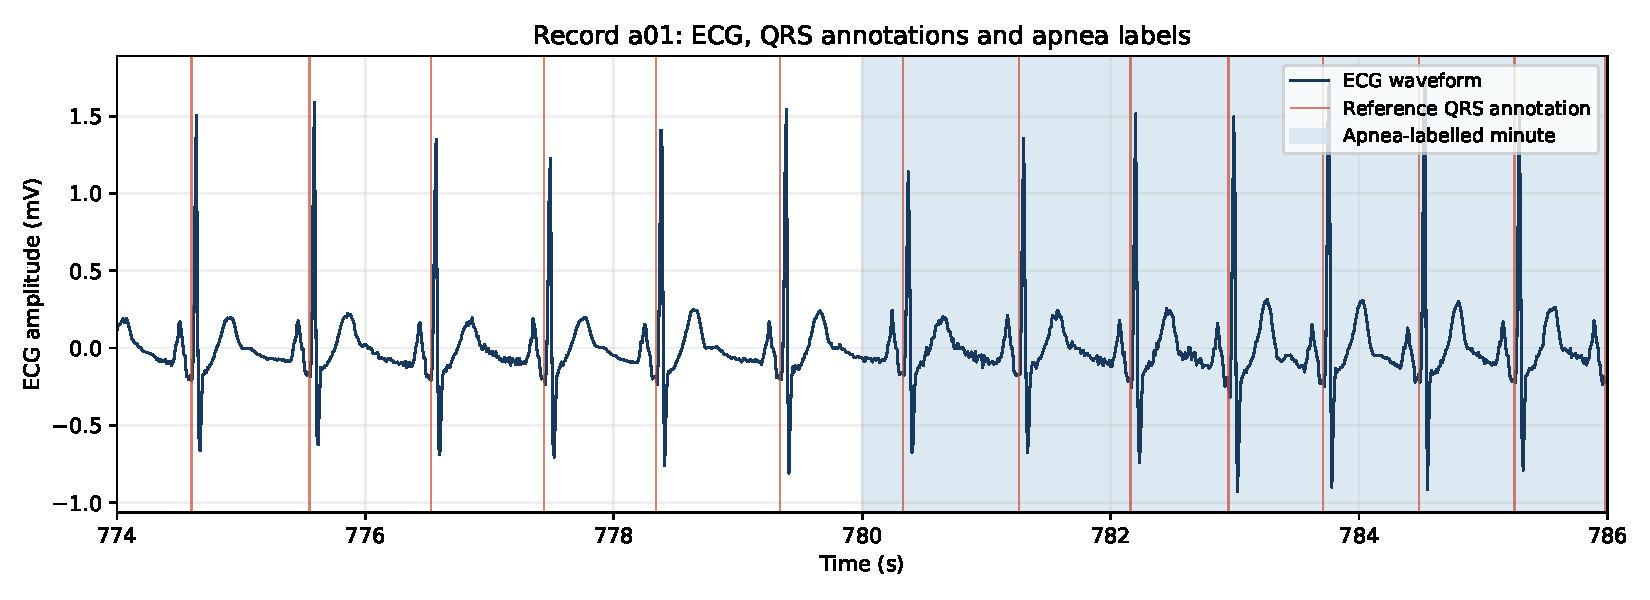
\includegraphics[width=0.95\linewidth]{figures/fig_ecg_annotations_a01.pdf}
\caption{ECG from a01 (774--786~s), with reference QRS events and blue shading for the apnea-labelled minute beginning at 780~s.}
\label{fig:ecg}
\end{figure}

\section{Adaptive R-peak detection and evaluation}
The detector applies a third-order Butterworth band-pass filter from 5 to 20~Hz in 60-s blocks with context padding. Taking the absolute filtered signal allows it to handle either ECG polarity. The local peak-height threshold is the larger of 40\% of the 99th amplitude percentile and four times the median amplitude. Peaks must also meet a prominence criterion and be separated by at least 0.35~s. These local thresholds allow the detector to adjust to amplitude changes across a recording. The waveform supplies all detection inputs; reference annotations are reserved for evaluation. Errors in beat detection can affect heart-rate-variability measurements \cite{weinstein2026}.

The two terms in the height rule respond to different features of the local amplitude distribution. The upper percentile follows the scale of large filtered excursions, while the median supplies a lower bound tied to the typical local amplitude. Peak prominence is set to 30\% of the resulting height threshold. Together with the minimum separation, these rules limit small excursions and closely spaced duplicate candidates. Their effectiveness is measured by the record-level results below.

Filtering uses forward and backward passes on padded blocks. The padding reduces the influence of an artificial block edge on candidates near a 60-s boundary. Only candidates in the central block are retained. After combining blocks, the detector compares adjacent candidates closer than the refractory separation and retains the stronger one. This final pass matters because thresholds are computed locally, so two neighbouring blocks can select different candidates around their shared boundary.

Detected and reference beats are matched one-to-one within a tolerance of $\pm0.12$~s. Matched pairs count as true positives (TP), unmatched detections as false positives (FP), and unmatched references as false negatives (FN). Precision, recall and F1 are
\begin{equation}
P=\frac{TP}{TP+FP},\qquad
R=\frac{TP}{TP+FN},\qquad
F_1=\frac{2TP}{2TP+FP+FN}.
\label{eq:f1}
\end{equation}
The matching tolerance allows for differences between the location of a QRS annotation and the detected amplitude maximum.

Precision and recall answer different practical questions. Precision describes how often a detection can be paired with a reference event; recall describes how often a reference event has a detection nearby. Reporting both makes excess detections and missed events visible even when their effects on the total beat count partly cancel. F1 combines the two counts in one score, and the timing-offset summaries describe where the matched detections occur relative to their references.

At 100~Hz, one sample corresponds to 10~ms, and the 0.12-s matching tolerance corresponds to 12 samples. This defines the time scale of the evaluation. The matching procedure walks through the two ordered event lists, using each event at most once. A cluster of detections near one reference can therefore contribute only one true positive; the remaining detections count as false positives.

\section{R--R intervals and cleaning}
For R-peak sample indices $p_i$ and ECG sampling frequency $f_s$, each interval is assigned to the midpoint of its two beats:
\begin{equation}
r_i=\frac{p_{i+1}-p_i}{f_s},\qquad
u_i=\frac{p_i+p_{i+1}}{2f_s}.
\label{eq:rr}
\end{equation}
The intervals $r_i$, measured in seconds, therefore occur at irregular times $u_i$. Cleaning removes intervals outside 0.35--2.00~s and those differing from an 11-point local median by more than 40\%. These heuristic rules exclude implausible or locally inconsistent intervals from subsequent analysis.

The midpoint convention places each measurement within the cardiac cycle whose duration it describes. Assigning intervals to consecutive beat numbers would instead treat short and long cardiac cycles as equally spaced in time. Spectral analysis needs the elapsed-time information, so all later stages retain the midpoint timestamps explicitly.

Missed and extra detections affect this representation in different ways. A missed beat combines two adjacent intervals into one longer interval. An extra beat splits an interval into two shorter ones. The absolute bounds remove extreme values, and the local-median rule responds to sudden departures from nearby intervals. A sustained detection error can also change the local median itself. For that reason, the cleaned sequence is inspected alongside the reference-derived sequence, and detection scores are reported separately.

For correctly paired consecutive beats, the effect of timing offsets has a simple form. Let the detected beat time be $\hat t_i=t_i+e_i$, where $e_i$ is its offset from the reference. The corresponding interval difference is
\begin{equation}
\hat r_i-r_i=e_{i+1}-e_i.
\label{eq:timing_propagation}
\end{equation}
A common shift in both beat times cancels. Changes in the shift remain in the interval sequence. This identity explains why matched-beat offsets and R--R errors need separate interpretation, especially when evaluating their effect on a later spectrum.

Variability is calculated from the retained intervals before interpolation. A 180-s window includes intervals whose midpoints satisfy $t_0\leq u_i<t_0+180$. For its $n$ retained intervals, the sample standard deviation in milliseconds is
\begin{equation}
s_{\mathrm{RR}}=1000\sqrt{\frac{1}{n-1}\sum_{i=1}^{n}(r_i-\bar r)^2},
\qquad \bar r=\frac{1}{n}\sum_{i=1}^{n}r_i.
\label{eq:rr_sd}
\end{equation}
I use the term cleaned-RR SD because the cleaning procedure filters interval values without classifying normal sinus beats. Group summaries report the median of these window-level standard deviations.

Using the intervals before interpolation keeps the variability calculation attached to the retained measurements. Interpolating to a denser grid changes the number and weighting of values in a standard-deviation calculation. The window-level definition also keeps each summary tied to a fixed 180-s period. Taking its group median gives each accepted window equal weight, regardless of how many beats it contains.

\section{Interpolation and spectral estimation}
\subsection{Representation on a regular grid}
A standard discrete Fourier transform requires equally spaced inputs. Linear or shape-preserving cubic (PCHIP) interpolation maps the retained R--R observations to a 4-Hz grid, $t_j=t_0+j/4$. This grid supplies the numerical inputs for spectral analysis; the underlying measurements remain the irregular R--R observations.

Between neighbouring retained measurements $(u_i,r_i)$ and $(u_{i+1},r_{i+1})$, linear interpolation uses
\begin{equation}
\tilde r(t)=(1-\lambda)r_i+\lambda r_{i+1},
\qquad \lambda=\frac{t-u_i}{u_{i+1}-u_i},\quad u_i\leq t\leq u_{i+1}.
\label{eq:linear_interpolation}
\end{equation}
Each predicted value is therefore determined by its two neighbours and its position between them. PCHIP uses piecewise cubic polynomials with continuous first derivatives and slopes chosen to preserve local monotonicity \cite{scipy_pchip}. It provides a smoother curve through the retained points. Comparing these methods tests whether that change in curve shape affects the selected spectral peak.

Values outside the observed time range and inside gaps longer than 3~s are initially marked as missing, while observed values at gap endpoints are retained. A window must contain at least 40 retained intervals and have at least 95\% valid grid coverage. Remaining missing values at the boundaries are filled with the nearest valid value. Windows with internal missing values are rejected.

Coverage and gap position are checked separately. A small internal gap can leave more than 95\% of the grid valid and still require rejection. Boundary gaps arise naturally because interval midpoints usually fall inside the window, leaving a short unsupported region before the first or after the last observation. Nearest-value filling handles those edges after the coverage check. Inside the window, the 3-s rule preserves the distinction between observed local variation and a long span with no retained support.

The 4-Hz spacing is 0.25~s, which supplies an analysis grid finer than the retained beat-to-beat observations. Increasing the grid density would create more interpolated values from the same measurements. In this study the grid frequency stays fixed, allowing the comparison to focus on interpolation shape and the subsequent spectral settings.

\subsection{Fourier representation and Welch settings}

For equally spaced values $x_j$ sampled at $f_g=4$~Hz, the discrete Fourier transform is
\begin{equation}
X_k=\sum_{j=0}^{N-1}x_j\exp(-2\pi\mathrm{i}jk/N),
\qquad f_k=\frac{k f_g}{N}.
\end{equation}
SciPy's Welch routine analyses the interpolated series using a periodic Hann window, a segment length of $\min(512,N)$ samples, 50\% overlap and linear detrending within each segment. The FFT length equals the segment length. A 180-s window contains $N=720$ grid points, so only one complete 512-point segment fits. With these settings, the routine returns a single modified periodogram covering the first 128~s. Shorter segments would allow averaging over several spectra, at the cost of wider frequency-bin spacing.

The DFT expresses variation as a combination of sinusoidal components at the frequencies $f_k$. A modified periodogram applies a taper before calculating the squared transform. The Hann taper reduces the weight of observations near segment edges, which changes how the finite observation interval contributes to the spectrum. Linear detrending first removes the fitted straight-line component within the segment. These operations define which variation enters the peak search.

Welch estimation averages modified periodograms from the complete overlapping segments \cite{scipy_welch}. For $N$ grid points, segment length $L$ and overlap $O$, the number of complete segments is
\begin{equation}
K=1+\left\lfloor\frac{N-L}{L-O}\right\rfloor.
\label{eq:welch_segments}
\end{equation}
Here $L=512$ and $O=256$, giving $K=1$. The final 208 grid points cannot form another complete segment under this configuration. The single-segment result is a consequence of the chosen parameters and remains relevant when comparing it with a method using observations across the full window.

The segment duration also determines the Fourier-bin spacing: $f_g/L=1/128$~Hz in this case. Shortening the segments increases the number that can be averaged and broadens this spacing. Extending the FFT through zero padding would evaluate the finite-data spectrum on a finer grid, while the segment duration would remain the same. The submitted configuration uses no zero padding.

\subsection{Lomb--Scargle on irregular observations}

Lomb--Scargle uses all retained irregular observations in the 180-s window. A least-squares linear trend is fitted against the observation times and subtracted. At each trial frequency, sine and cosine terms are fitted to the residuals at their original timestamps. The periodogram uses 601 equally spaced frequencies from 0.10 to 0.40~Hz, a spacing of 0.0005~Hz, with \texttt{normalize=True}.

Writing the detrended observations as $z_i$, the sinusoidal fit at a trial frequency $f$ minimises
\begin{equation}
Q_f(a,b)=\sum_i\left[z_i-a\cos(2\pi f v_i)-b\sin(2\pi f v_i)\right]^2,
\qquad v_i=u_i-u_1.
\label{eq:lomb_fit}
\end{equation}
The timestamps enter this fit directly. Frequencies whose fitted sine and cosine terms explain more of the residual variation receive greater periodogram power \cite{scipy_lomb}. The implementation removes the intercept and linear trend before calling the routine and uses its default fixed zero offset for the residual model.

The distinction from Welch involves more than the sampling grid. Welch detrends and tapers an interpolated 128-s segment. Lomb--Scargle fits the irregular residuals across the 180-s window. Their displayed spectra are each divided by their own maximum within the search band. This makes peak locations and shapes easy to compare; the two plotted heights use separate scales.

\subsection{Numerical checks and peak selection}

Before selecting a peak, the implementation checks for finite inputs and rejects numerically negligible variation after detrending. This check covers both the irregular observations and the segments used by Welch. The spectra must also have finite values and positive power within the search band. These checks prevent constant or numerically degenerate inputs from receiving an arbitrary frequency.

The numerical floor is $100\epsilon\max(1~\mathrm{s},\max_i|r_i|)$, where $\epsilon$ is floating-point machine precision and the residuals are measured in seconds. If all detrended residuals are at or below this scale, the calculation stops before peak selection. The same check is applied to the segments that Welch actually uses. Checking those segments matters when variation occurs only in a later part of the window that the current Welch configuration omits.

For each method, the candidate frequency $f_*$ is the location of the largest spectral value in the 0.10--0.40~Hz search band. In cycles per minute,
\begin{equation}
\widehat{b}=60f_*.
\end{equation}
The band spans 6--24~cycles/min and sets the range examined in this exploratory analysis. Welch evaluates bins spaced by $60\times4/512=0.46875$~cycles/min; the Lomb--Scargle grid spacing is $60\times0.0005=0.03$~cycles/min. Grid spacing specifies where the spectrum is evaluated, while estimation accuracy also depends on the observations and the method. I count two estimates as consistent when they differ by at most 1~cycle/min. This descriptive threshold summarises agreement between methods.

The threshold is about two Welch bins under the default settings. It provides a readable summary of whether two methods select nearby parts of the search band. A difference larger than this threshold directs attention to a sensitive window. The analysis retains the actual frequency differences as well as these counts, so large discrepancies remain visible.

\section{Validation and study design}
The interpolation test uses a01 from 660 to 840~s. Every seventh R--R observation is withheld and predicted from the remaining points. A constant equal to the training mean, linear interpolation and PCHIP are evaluated at the same 28 held-out timestamps. For predictions $\hat r_i$ and observations $r_i$, the root mean squared error is
\begin{equation}
\operatorname{RMSE}=\sqrt{\frac{1}{m}\sum_{i=1}^{m}(\hat r_i-r_i)^2}.
\end{equation}

The holdout positions are fixed by their order in the interval sequence, making the comparison repeatable. Evaluation points must lie between retained training observations whose separation satisfies the gap rule. All three methods therefore predict the same safely interpolable observations. The constant-mean baseline describes the error obtained by using a typical interval throughout the window; improvement over it measures the value of following local interval changes. Mean absolute error (MAE) is also reported to show the typical error magnitude with less emphasis on the largest residuals.

Synthetic beat times provide a check with known modulation frequencies:
\begin{equation}
\tau_0=0,\qquad
\tau_{k+1}=\tau_k+0.82+0.07\sin(2\pi f_0\tau_k),
\label{eq:synthetic_beats}
\end{equation}
where time is in seconds and $f_0\in\{0.15,0.22,0.32\}$~Hz, corresponding to 9.0, 13.2 and 19.2~cycles/min. The baseline interval is 0.82~s and the modulation amplitude is 0.07~s. Beat times are generated until the final beat exceeds 240~s, rounded to the nearest millisecond, and passed through the same R--R construction and cleaning procedure. Spectral estimation uses the interval from 10 to 190~s. These sequences contain no added random noise, so they test frequency recovery under idealised conditions.

Generating beat times recursively keeps the observation times dependent on the modulated intervals. The synthetic input therefore exercises the midpoint representation and resampling stages as well as the spectral calculation. Its known frequency gives a direct numerical target. Rounding and finite windowing remain part of the calculation, while noise, competing frequencies and detector errors are left for future robustness experiments.

The real-data comparison uses four records with apnea annotations: a05, a10, b05 and c01. Each record is divided into disjoint 180-s windows. Eligible windows have the same label throughout, either normal or apnea. Up to four windows per available class and record are selected at positions spread across the recording, then assessed using the quality checks above. This stratified selection provides a descriptive comparison within records.

Window starts and durations align to complete minutes. A window is normal only when all three minute labels are normal, and apnea-labelled only when all three indicate apnea. Mixed or missing labels exclude a window from the class comparison. If more than four eligible windows exist in a class, selection is deterministic and spread across their ordered start times. Quality rejection occurs after selection; a rejected window is recorded rather than replaced by another candidate.

The separate QRS benchmark covers eight records (Table~\ref{tab:qrs}). Record a10 appears only in the window analysis, where its intervals undergo the same cleaning and spectral checks as the other records. For all four records, I also compare spectral peaks obtained from detected beats with those obtained from reference QRS positions.

\section{Computational organisation}
The software separates file reading, peak detection, interval analysis and window selection into modules. Stage scripts produce the saved results, while the main driver executes the stages and generates the LaTeX tables from CSV files. This structure lets an unexpected result be traced from a report value back to a window, an interval sequence and its detected beat times.

The loader retains the full ECG record in memory. Block filtering limits the additional arrays used during detection to the local padded block. One-to-one matching then advances through the ordered detection and reference lists, so its work grows linearly with their combined length. Spectral calculations operate on individual windows: the default interpolated input has 720 values, and Lomb--Scargle evaluates 601 trial frequencies for the retained observations. Selecting a small set of windows keeps the exploratory comparisons manageable while preserving their exact start times for inspection.

The 35 automated tests check file decoding, peak detection and matching, interval construction, gap handling, spectral recovery and window selection. They also cover numerical edge cases and output bookkeeping. Before a repeat run, known generated outputs are invalidated, and stage metadata records the parameters and success status. An empty rejection list still produces a CSV with its declared columns. These details keep a new run from appearing complete because files from an earlier run remain in the output directory.

\chapter{Results}
\label{ch:results}
\section{QRS detection varies across records}
The detector achieved an F1 score of 0.999967 on a01, with two unmatched detections and no missed reference beats (Table~\ref{tab:qrs}). Figure~\ref{fig:peakmatch} shows an example from this record. Performance was lower on a02 and b05, with F1 scores of 0.902031 and 0.912905. The main issue in a02 was excess detections: 7,548 FP compared with 72 FN. In b05, both types of error were common, with 2,092 FP and 2,682 FN.

For matched beats, the median signed timing offset (detected time minus reference time) ranged from 30 to 50~ms across records. The 95th percentile of the absolute offset ranged from 40 to 80~ms, reaching 80~ms in b05. A fixed timing shift cancels when consecutive beat times are subtracted to form an R--R interval; changes in that shift affect the interval value.

\begin{figure}[htbp]
\centering
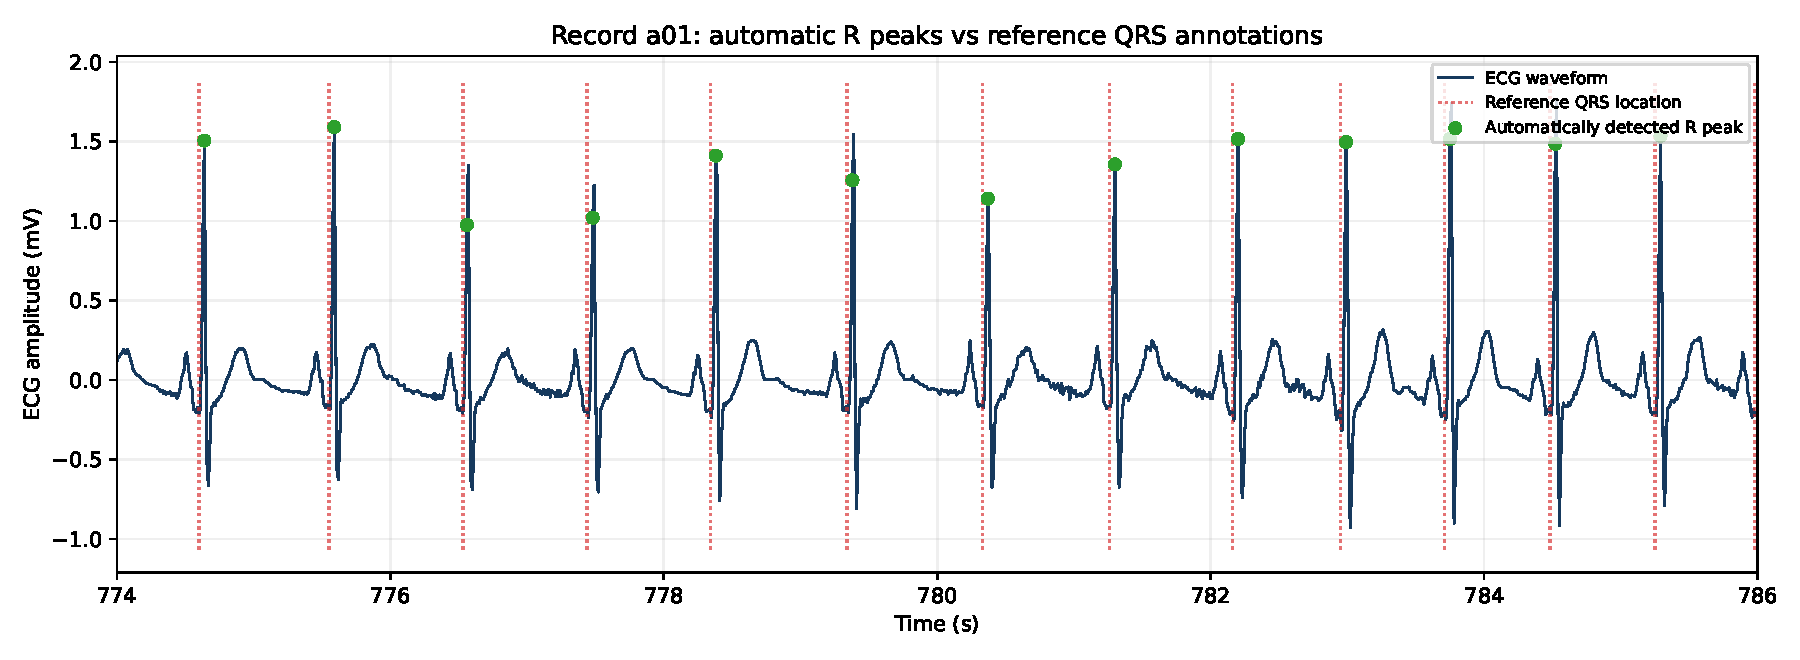
\includegraphics[width=0.92\linewidth]{figures/fig_r_peak_detection_a01.pdf}
\caption{Detected R peaks (green markers) and reference QRS events (red lines) in a01 from 774 to 786~s.}
\label{fig:peakmatch}
\end{figure}
\begin{table}[htbp]
\centering
\small
\begin{tabular}{lrrrrrr}
\toprule
Record & TP & FP & FN & Precision & Recall & F1 \\
\midrule
a01 & 29,938 & 2 & 0 & 0.9999 & 1.0000 & 1.0000 \\
a02 & 35,080 & 7,548 & 72 & 0.8229 & 0.9980 & 0.9020 \\
a05 & 28,726 & 37 & 33 & 0.9987 & 0.9989 & 0.9988 \\
b01 & 35,060 & 33 & 31 & 0.9991 & 0.9991 & 0.9991 \\
b05 & 25,020 & 2,092 & 2,682 & 0.9228 & 0.9032 & 0.9129 \\
c01 & 27,535 & 90 & 175 & 0.9967 & 0.9937 & 0.9952 \\
c05 & 27,906 & 172 & 98 & 0.9939 & 0.9965 & 0.9952 \\
x01 & 36,453 & 145 & 8 & 0.9960 & 0.9998 & 0.9979 \\
\bottomrule
\end{tabular}
\caption{R-peak detection scores against the supplied machine-generated QRS annotations for 8 records. Detections and references are matched within $\pm 0.12$~s.}

\label{tab:qrs}
\end{table}


The error balance differs between the two difficult records. Recall in a02 remained high at 0.9980, while precision fell to 0.8229. In b05, precision and recall were both lower, at 0.9228 and 0.9032. This distinction matters for interval construction: excess detections create short intervals, whereas missed events create longer combined intervals.

Total beat counts alone hide much of this behaviour. In b05, 27,112 detections were compared with 27,702 references, a difference of 590. The one-to-one evaluation nevertheless counted 4,774 unmatched events in total: 2,092 detections and 2,682 references. The similar overall counts therefore coexist with substantial local disagreement. Table~\ref{tab:timing} adds the timing information for the matched events.
\begin{table}[htbp]
\centering
\begin{tabular}{lrr}
\toprule
Record & Median signed offset (ms) & 95th absolute percentile (ms) \\
\midrule
a01 & 40 & 40 \\
a02 & 30 & 40 \\
a05 & 40 & 50 \\
b01 & 40 & 50 \\
b05 & 40 & 80 \\
c01 & 50 & 50 \\
c05 & 50 & 50 \\
x01 & 50 & 50 \\
\bottomrule
\end{tabular}
\caption{Timing offsets among matched detected and reference beats. Signed offsets are detected time minus reference time; each row summarises one recording.}
\label{tab:timing}
\end{table}


The median offsets were positive in all eight records. For a01, the median and 95th absolute percentile were both 40~ms; b05 had the same median but an 80-ms absolute percentile. Equation~\ref{eq:timing_propagation} shows why the temporal variation in these offsets is relevant to R--R analysis. The current summaries describe their distributions across each record. Locating abrupt changes in offset would require a further comparison of successive matched beat pairs.

\section{R--R construction and interpolation checks}
For a01, the detector found 29,940 R peaks. Of the resulting 29,939 intervals, 29,903 passed cleaning (99.88\%). Figure~\ref{fig:rr} compares the cleaned interval sequences obtained from detected and reference beats.

\begin{figure}[htbp]
\centering
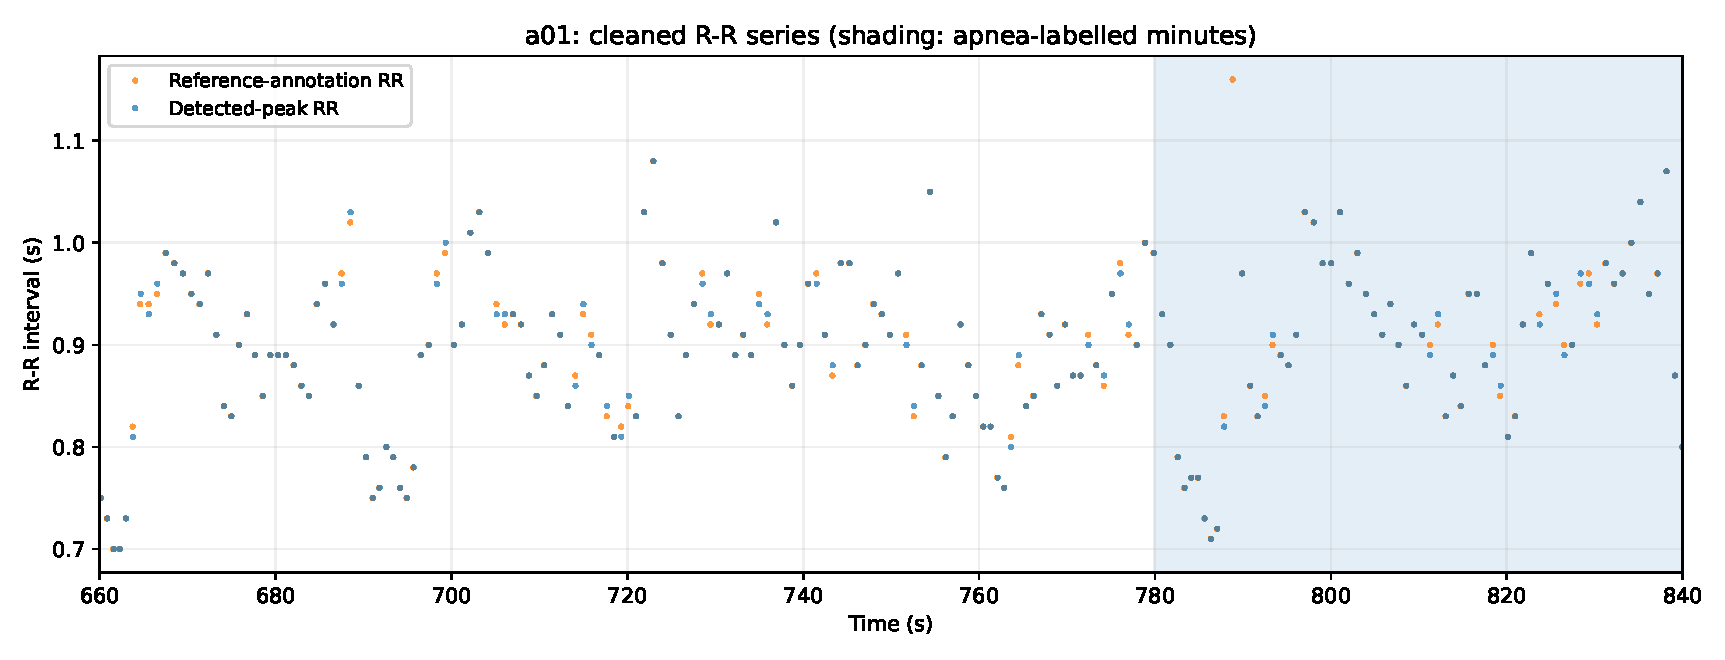
\includegraphics[width=0.95\linewidth]{figures/fig_rr_tachogram_a01.pdf}
\caption{Cleaned R--R intervals from detected beats and reference QRS events in a01 (660--840~s). Shading marks apnea-labelled minutes.}
\label{fig:rr}
\end{figure}

Both interpolation methods reconstructed held-out observations more accurately than the constant-mean baseline (Table~\ref{tab:interpolation}). RMSE fell from 83.22~ms to 36.17~ms with linear interpolation and 35.61~ms with PCHIP. The improvement was similar for the two methods in this window.
\begin{table}[htbp]
\centering
\begin{tabular}{lrrr}
\toprule
Reconstruction method & RMSE (ms) & MAE (ms) & Held-out points \\
\midrule
Constant-mean baseline & 83.22 & 64.72 & 28 \\
Linear & 36.17 & 29.29 & 28 \\
PCHIP & 35.61 & 28.27 & 28 \\
\bottomrule
\end{tabular}
\caption{Reconstruction errors for 28 held-out R--R observations in a01 (660--840~s). Holdout stride 7; all methods are evaluated at the same timestamps.}

\label{tab:interpolation}
\end{table}


The MAE results follow the same ordering: 64.72~ms for the constant baseline, 29.29~ms for linear interpolation and 28.27~ms for PCHIP. Thus the improvement is visible in both error measures. PCHIP's RMSE advantage over linear interpolation is only about 0.56~ms in this test. That small difference, measured in one window, gives little reason to prefer the more complex interpolator for all records.

Figure~\ref{fig:interpolation} displays the reconstruction errors using the saved results from the same holdout test. The comparison concerns interval values between nearby observations. It is most informative about the local reconstruction step and the benefit of following changes through time.
\begin{figure}[htbp]
\centering
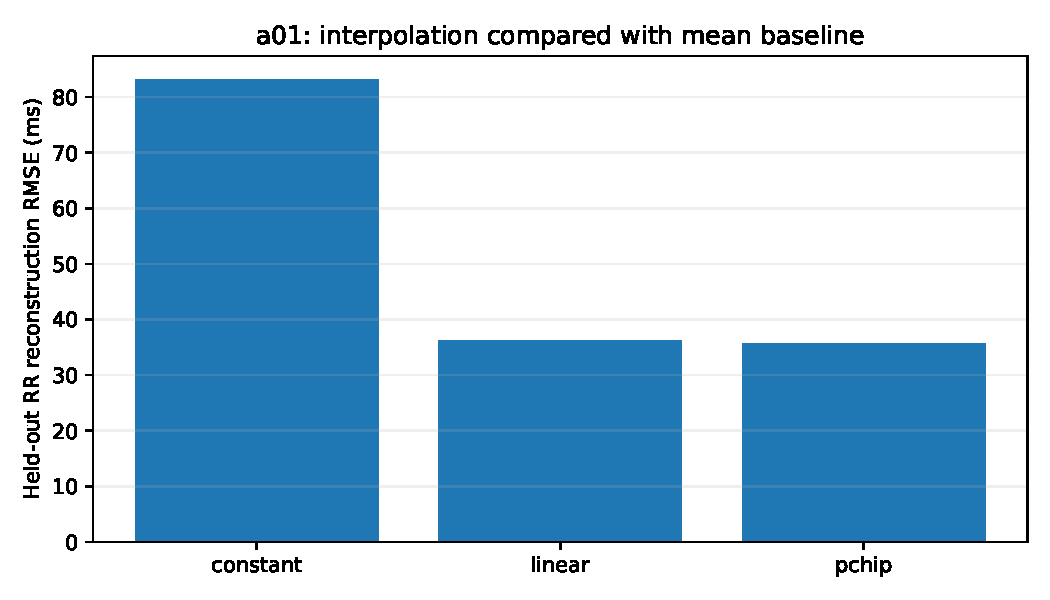
\includegraphics[width=0.80\linewidth]{figures/fig_interpolation_validation_a01.pdf}
\caption{RMSE for the 28 held-out R--R observations in a01. The plotted values are the same reconstruction errors reported in Table~\ref{tab:interpolation}.}
\label{fig:interpolation}
\end{figure}

\section{Recovery of known synthetic frequencies}

Both spectral methods also recovered the three synthetic modulation frequencies closely (Table~\ref{tab:synthetic}). Welch's absolute errors ranged from 0.019 to 0.094~cycles/min. Lomb--Scargle selected the imposed frequencies, all three of which lie on its search grid.
\begin{table}[htbp]
\centering
\begin{tabular}{rrrr}
\toprule
Known (cycles/min) & Welch & Lomb--Scargle & Welch abs. error \\
\midrule
9.0 & 8.91 & 9.00 & 0.094 \\
13.2 & 13.12 & 13.20 & 0.075 \\
19.2 & 19.22 & 19.20 & 0.019 \\
\bottomrule
\end{tabular}
\caption{Recovered spectral peaks for 3 synthetic modulation frequencies. All frequencies and errors are in cycles/min.}

\label{tab:synthetic}
\end{table}


The Welch estimates lie on the Fourier grid defined by its 512-point segment. The small residual errors are consistent with selecting nearby discrete bins. Lomb--Scargle evaluates each of the three imposed frequencies directly because they lie on its search grid. The exact displayed matches therefore have a straightforward numerical explanation.

These tests also connect the implementation stages. A wrong conversion between hertz and cycles per minute, a loss of elapsed-time information in the R--R timestamps, or an unsuitable spectral input could affect recovery of the imposed modulation. Close recovery supports this part of the calculation under the specified inputs. The experiment covers three single-frequency, noise-free cases; robustness to more complicated interval behaviour is considered in the discussion.

\section{Spectral estimates and method sensitivity}
In a01 from 660 to 840~s, Welch selected 9.84~cycles/min and Lomb--Scargle selected 6.42~cycles/min (Figure~\ref{fig:spectra}). The four-record analysis compares peak locations across a wider set of windows.

\begin{figure}[htbp]
\centering
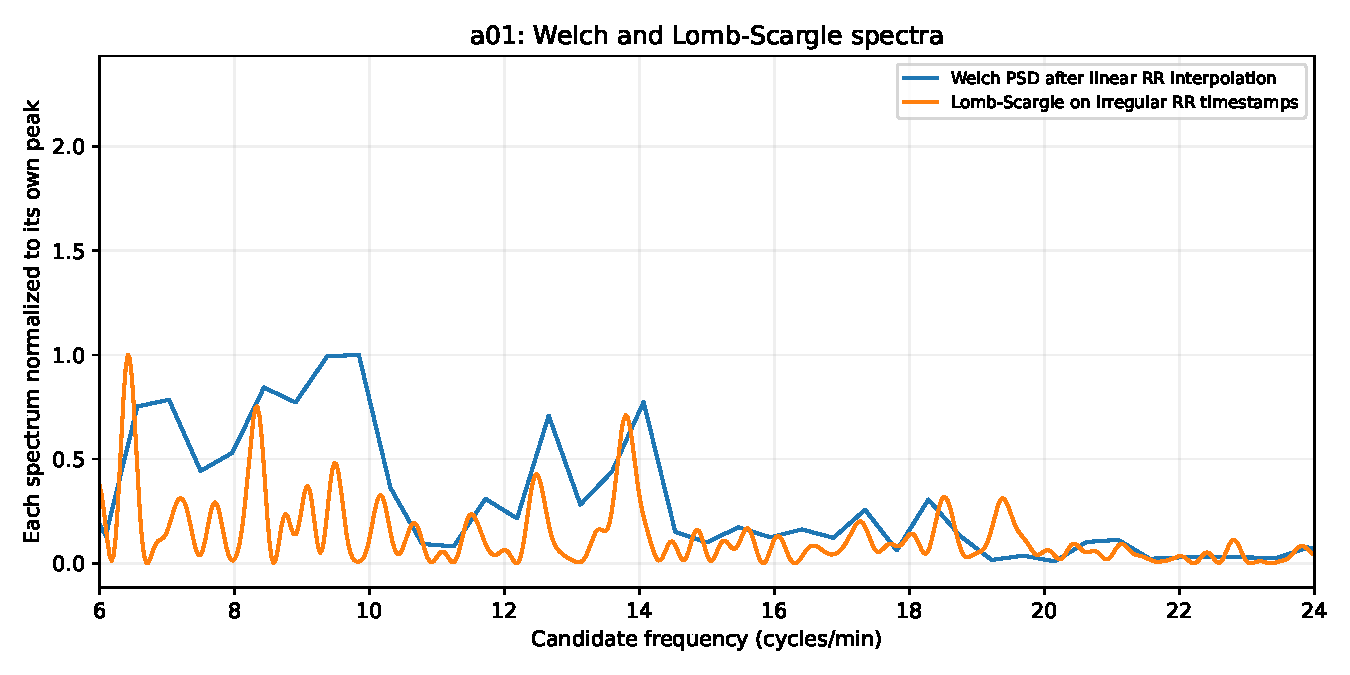
\includegraphics[width=0.80\linewidth]{figures/fig_rr_spectra_a01.pdf}
\caption{Spectra for a01 (660--840~s), each normalised to its maximum within the search band. Welch uses the first 128~s of the interpolated grid; Lomb--Scargle uses retained observations across 180~s. Normalisation supports comparison of spectral shape and peak location.}
\label{fig:spectra}
\end{figure}

Of 28 selected windows, 24 passed the quality checks; reasons were recorded for the four exclusions. Linear and PCHIP Welch peaks agreed within 1~cycle/min in 22 windows, while detected and reference beats gave peaks within this threshold in 23 (Table~\ref{tab:consistency}). The latter estimates were identical in all eight accepted a10 windows.

The two interpolation exceptions were large. The b05 window starting at 23,400~s gave 7.97~cycles/min with linear interpolation and 12.66~cycles/min with PCHIP, a difference of 4.69~cycles/min. The c01 window starting at 19,260~s gave 6.56 and 13.59~cycles/min, a difference of 7.03~cycles/min.

Welch and Lomb--Scargle agreed within 1~cycle/min in 17 windows. Their configurations differ in time coverage, detrending, windowing and frequency grids. Figure~\ref{fig:sensitivity} compares these differences with those from detected versus reference beats.
\begin{table}[htbp]
\centering
\begin{tabular}{lr}
\toprule
Comparison & Windows with $\leq 1$ cycle/min difference \\
\midrule
Linear vs PCHIP (Welch) & 22 / 24 \\
Detected R peaks vs reference QRS (Welch) & 23 / 24 \\
Welch vs Lomb--Scargle & 17 / 24 \\
\bottomrule
\end{tabular}
\caption{Frequency agreement across the 24 accepted 180-s windows, using an absolute difference of at most 1~cycle/min.}

\label{tab:consistency}
\end{table}


\begin{figure}[htbp]
\centering
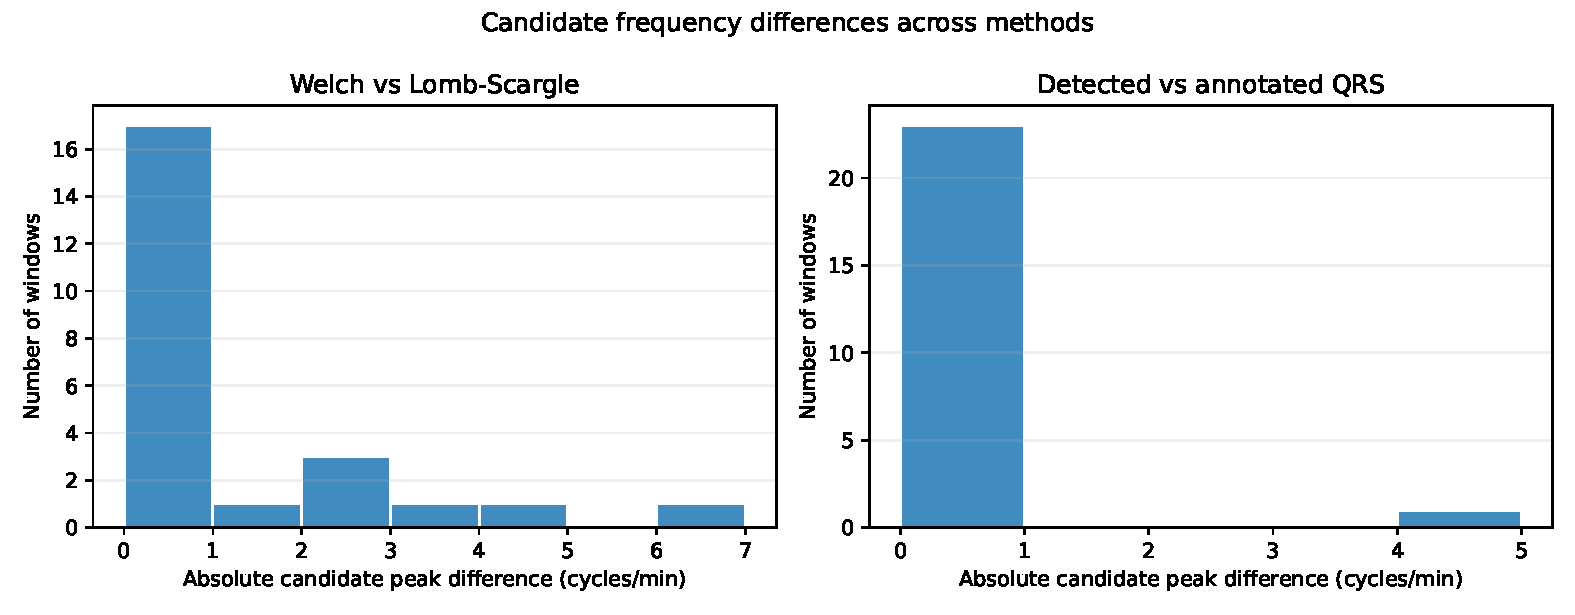
\includegraphics[width=0.78\linewidth]{figures/fig_method_sensitivity.pdf}
\caption{Absolute differences in candidate peak frequency across the 24 accepted windows: Welch versus Lomb--Scargle (left), and detected versus reference beats using Welch (right).}
\label{fig:sensitivity}
\end{figure}

\FloatBarrier
\section{Window acceptance and rejection}
The accepted sample contains eight windows each from a05 and a10, six from b05 and two from c01. The four exclusions in Table~\ref{tab:rejected} explain how the selected set changed after quality control. Two windows failed the grid-coverage threshold, one contained an unresolved internal gap, and one had too few retained intervals for spectral analysis.
\begin{table}[htbp]
\centering
\small
\begin{tabular}{llrl}
\toprule
Record & Label & Start (s) & Recorded reason \\
\midrule
b05 & Normal & 7,560 & Valid grid coverage 46.5\% \\
b05 & Apnea & 19,260 & Unresolved internal gap \\
c01 & Normal & 0 & Fewer than 40 retained intervals \\
c01 & Normal & 28,800 & Valid grid coverage 92.8\% \\
\bottomrule
\end{tabular}
\caption{Selected 180-s windows excluded by the quality checks. Coverage percentages are the rounded values recorded by the software.}
\label{tab:rejected}
\end{table}


The b05 window starting at 7,560~s had only 46.5\% valid grid coverage, while the c01 window at 28,800~s had 92.8\%. Both fall below the stated 95\% requirement despite their very different amounts of missing support. The internal-gap rejection in b05 shows why coverage is checked together with the location of missing values. The software records the first failed condition encountered while evaluating the window; the table reports that condition without assigning an unexamined waveform cause.

These exclusions are part of the result because consistency is calculated only for accepted windows. The 24 successful cases therefore describe data that satisfied all the implemented comparisons. Retaining the rejected start times makes it possible to inspect what the screening process leaves out and to reproduce the denominator used in the agreement counts.

\section{Normal and apnea-labelled windows}
Median cleaned-RR SD was higher in the apnea-labelled group in each record with both classes (Table~\ref{tab:windows}). Normal and apnea medians were 48.7 and 97.2~ms in a05, 50.8 and 79.3~ms in a10, and 67.6 and 98.3~ms in b05. Each group contained three or four windows. Record c01 contributed two normal windows and no apnea windows. Figure~\ref{fig:labels} shows the candidate Welch frequencies for these same groups.

\begin{figure}[htbp]
\centering
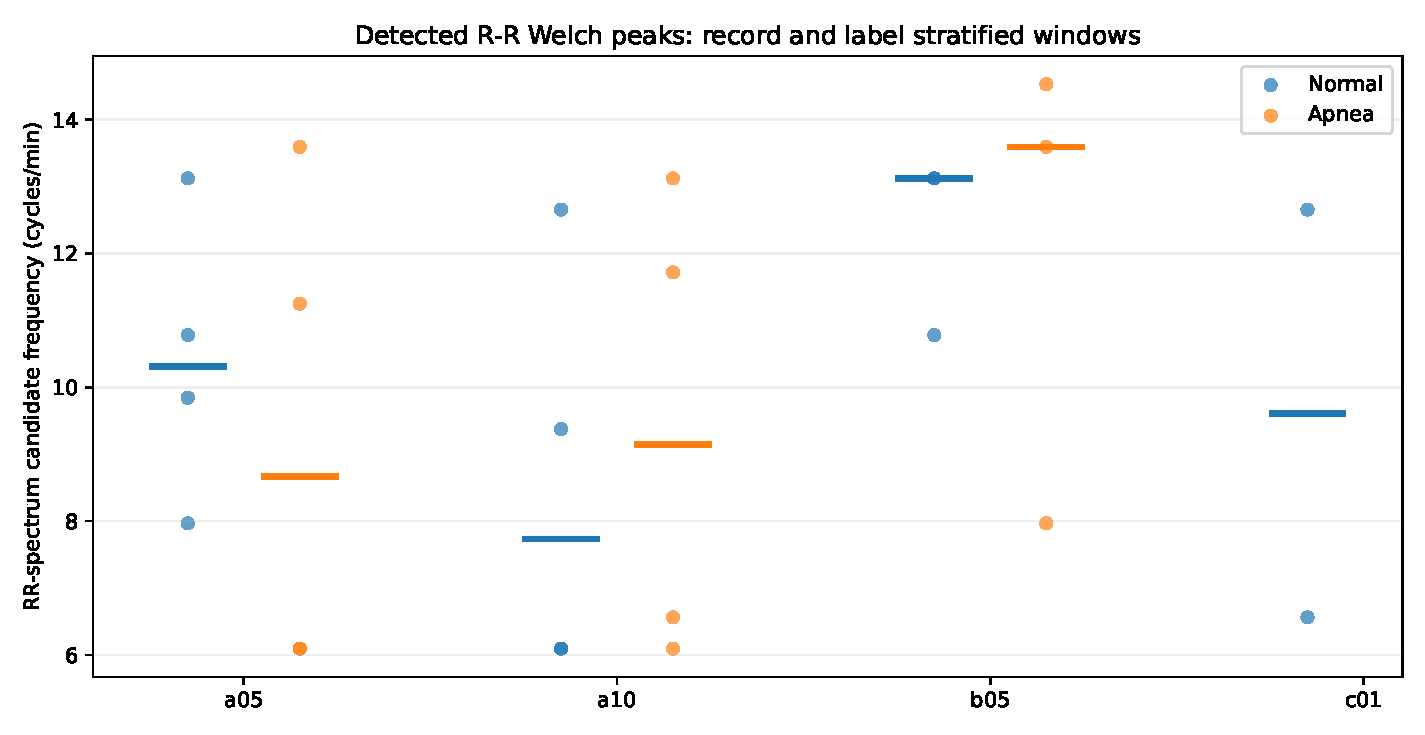
\includegraphics[width=0.92\linewidth]{figures/fig_candidate_frequency_by_label.pdf}
\caption{Candidate Welch frequencies in the selected normal and apnea-labelled windows. Each point represents a 180-s window; horizontal marks indicate group medians within each record.}
\label{fig:labels}
\end{figure}
\begin{table}[htbp]
\centering
\small
\begin{tabular}{llrrrr}
\toprule
Record & Label & $n$ windows & Cleaned-RR SD (ms) & Welch & Lomb \\
\midrule
a05 & Normal & 4 & 48.7 & 10.31 & 10.20 \\
a05 & Apnea & 4 & 97.2 & 8.67 & 9.98 \\
a10 & Normal & 4 & 50.8 & 7.73 & 7.97 \\
a10 & Apnea & 4 & 79.3 & 9.14 & 8.61 \\
b05 & Normal & 3 & 67.6 & 13.12 & 13.29 \\
b05 & Apnea & 3 & 98.3 & 13.59 & 13.89 \\
c01 & Normal & 2 & 73.2 & 9.61 & 13.02 \\
\bottomrule
\end{tabular}
\caption{Group medians of window-level cleaned-RR SD and candidate frequency (cycles/min) for selected 180-s windows. Variability is calculated from the retained R--R intervals before interpolation.}

\label{tab:windows}
\end{table}


\begin{samepage}
Variability and peak frequency show different patterns across the groups. Cleaned-RR SD was higher in all three paired apnea comparisons. The median Welch frequency fell from 10.31 to 8.67~cycles/min in a05, rose from 7.73 to 9.14~cycles/min in a10, and rose from 13.12 to 13.59~cycles/min in b05. The relationship between interval variability and the location of the largest peak varied across these records.
\par
\end{samepage}

The group sizes also differ after rejection. Each a05 and a10 group contains four windows, each b05 group contains three, and c01 has only two normal windows. Comparing records separately preserves this structure. The group medians summarise the observed windows while the individual points in Figure~\ref{fig:labels} retain the within-group spread.
\FloatBarrier

\chapter{Discussion}
\label{ch:discussion}
\section{Detection errors and downstream agreement}
Detection performance varied enough across records to affect the interpretation of the later stages. Local thresholds handled a01 well, while a02 produced many excess detections and b05 had both excess and missed detections. These errors can change individual R--R intervals and introduce artificial variation. The reference annotations also carry uncertainty. Examining failure segments in a02 and b05 would help identify which waveform features cause the detector to fail; the current scores show the extent of the problem but leave its cause unresolved.

Plotting periods with concentrated unmatched detections or references alongside the filtered waveform and threshold would distinguish persistent problems from short bursts of poor detection. Such failure plots would complement the high-scoring a01 example and help explain the differences between records.

The strong detected-versus-reference frequency agreement in the accepted windows is useful downstream evidence. It indicates that, in most selected cases, replacing the beat source preserved the largest Welch peak within the chosen tolerance. Peak selection compresses a whole interval sequence into one number, however. Different interval errors can leave that number unchanged. The beat-level results and the window-level frequency comparison consequently describe different aspects of the workflow and are most informative when read together.

\section{Interpolation and sensitive peak locations}

Reconstruction error and peak location depend on different features of the signal. RMSE averages squared discrepancies at the held-out timestamps. The peak rule selects whichever evaluated frequency has the greatest power. If two separated spectral peaks have similar heights, a modest change in the interpolated curve can change which one is selected. This gives a possible explanation to investigate in the b05 and c01 exceptions. Identifying the mechanism requires examining their interval sequences and full spectra.

For those two cases, overlaying the interpolants and their full spectra with the other settings fixed would show where the curves differ and whether peak selection shifts locally or switches between separated candidates. This would focus the investigation on the large differences already present in the results.

\section{What the spectral comparison establishes}

Welch used one 128-s segment and Lomb--Scargle used observations across 180~s, with different detrending, windowing and frequency grids. A controlled comparison should align the time range, then vary segment length and detrending separately. Comparing a full-window periodogram with several shorter Welch segments would clarify the trade-off between frequency spacing and averaging.

Time coverage is especially relevant when interval behaviour changes within a window. A fluctuation appearing mainly in the final part of a 180-s window can influence the Lomb--Scargle fit while contributing no samples to the current Welch segment. The Hann taper also gives unequal weight to different positions within that segment. These are concrete differences in the information used by the two calculations. Their effects on the observed discrepancies remain to be separated by a controlled experiment.

The finer Lomb--Scargle grid should also be read in the context of the finite data. It evaluates candidate frequencies more densely, while the available observation interval and the structure of the signal still constrain interpretation. The synthetic matches are useful checks of recovery on that grid. The real-data disagreement identifies windows whose dominant frequency depends on the implemented configuration.

\section{When a candidate deserves further interpretation}

The quality checks address missing observations and numerical degeneracy. A separate question is whether a valid window contains a distinct periodic component. The current peak rule can still select a maximum in noise or weakly structured data, so a validated measure of peak quality would improve the interpretation. The fixed 6--24~cycles/min band also limits which periodicities can be found. Testing noise levels, modulation amplitudes and frequencies outside this range would help define where the method is useful.

The evidence can be assessed in a practical order. First, check whether a window has enough retained observations and acceptable support. Next, inspect whether its spectrum contains a distinct peak and whether that peak is stable across reasonable processing choices. Finally, compare its frequency with an independently measured respiratory signal. The present workflow implements the support checks and several consistency comparisons. Numerical rejection of a constant input addresses the first part of this sequence; a confidence rule for noisy periodic structure still needs validation.

This order also clarifies how to extend the synthetic study. A sequence with a known frequency and progressively smaller modulation would test when a candidate becomes unstable. Pure noise would test how often a peak-quality rule accepts a signal without an imposed periodic component. Missed or extra synthetic beats would connect detection errors to the downstream estimate.

\begin{samepage}
\section{Sampling and physiological interpretation}

The apnea comparison contains few repeated windows from each record. Its variability patterns warrant follow-up with more subjects. Independent respiratory validation is needed to connect the spectral peaks to breathing rate. This study analysed ECG and minute-level apnea labels. Some Apnea--ECG records include additional respiratory channels \cite{penzel2000}; comparing suitable synchronised windows would directly assess the physiological meaning of the extracted frequencies.
\par
\end{samepage}

Selecting homogeneous labelled windows makes the group definition clear and excludes transitions between minute-level states. It also means that the analysis describes the chosen stable-label periods. Spreading the windows across a record provides temporal coverage, while repeated windows from one recording remain clustered observations. A larger study should preserve the subject as the unit for assessing generalisation and should report how quality rejection changes the available sample in each class.

An external respiratory comparison would need its own explicit procedure. Suitable channels would first be checked for synchronisation and signal quality. A reference frequency would then be extracted over the same accepted time windows using rules set in advance. Reporting absolute frequency differences, rejected windows and difficult examples would connect the numerical consistency results to respiratory interpretation. This would extend the present analysis from reproducible candidate extraction to direct evaluation against a physiological measurement.

\chapter{Conclusion}
\label{ch:conclusion}
I developed a reproducible workflow that detects R peaks, constructs cleaned R--R intervals and extracts candidate periodicities in the 6--24~cycles/min band. Detection performance varied across the eight benchmark records. Interpolation reduced held-out reconstruction error to about 36~ms, and both spectral methods recovered the three imposed synthetic frequencies closely.

Across 24 accepted real-data windows, linear and PCHIP interpolation usually gave similar Welch peaks, with two substantial exceptions. Welch and Lomb--Scargle differed more often under the chosen settings. The next priorities are to explain the sensitive windows, compare spectral configurations under matched conditions, and validate the candidate frequencies against synchronised respiratory signals.

The existing results identify where further work would be most informative: a02 and b05 for detector failures, the two interpolation-sensitive windows for peak instability, and the Welch configuration for the interaction between time coverage and segmentation. Addressing these cases would strengthen the explanation of the results while keeping the analysis tied to observations already available in the project.

\section*{Code and data reproducibility}
\phantomsection
\addcontentsline{toc}{section}{Code and data reproducibility}
The companion software archive includes the Python source, \texttt{requirements.txt}, 35 automated tests and the reproduction driver \texttt{run\_all.py}. Place the separately supplied \texttt{data.zip} beside the scripts and run \texttt{python run\_all.py} to regenerate the figures, CSV results and all seven LaTeX table fragments. The software \texttt{README.md} documents the data source, package versions, command-line options and the scripts responsible for each output. Table values in this report come from the saved analysis CSVs.
